\subsection{Capacidade de Canal}

% bilmes Homework 5 - q1

\begin{questions}
\question{
Determine a capacidade dos seguintes canais:

\begin{parts}
\part 

Dois canais binários simétricos.
\begin{figure}[h!]
\centering
\includegraphics[width=0.2\linewidth]{../images/2paralell_binarychannel.pdf}
\caption{Dois canais binários simétricos.}
\label{fig:q1a}
\end{figure}


\part 

Um canal binário simétrico e um único símbolo.
\begin{figure}[h!]
\centering
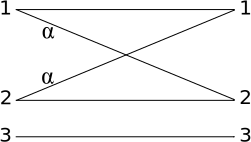
\includegraphics[width=0.2\linewidth]{../images/singlechannel_binarychannel.pdf}
\caption{Um canal binário simétrico e um único símbolo.}
\label{fig:q1b}
\end{figure}


\part 

Um canal binário simétrico e um canal ternário.
\begin{figure}[h!]
\centering
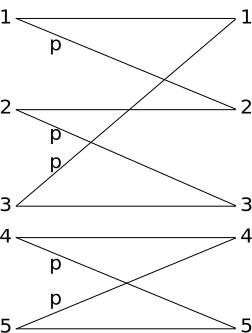
\includegraphics[width=0.2\linewidth]{../images/ternarychannel_binarychannel.pdf}
\caption{Um canal binário simétrico e um canal ternário.}
\label{fig:q1a}
\end{figure}



\part 

Um canal ternário.
\begin{equation}
        p(y\vert x) = \begin{bmatrix} 2/3 & 1/3 & 0 \\ 0 & 1/3 & 2/3 \end{bmatrix}
\end{equation}

\end{parts}

}


\begin{solution}
\begin{parts}
\part 

Temos um canal com $\mathcal{X} = \mathcal{Y} = \{1, 2, 3, 4\}$, alfabeto de entrada e saída.
A matriz de transição do canal é dada por

  \begin{equation}
  p(y|x) = 
  \begin{pmatrix}
  1-p & p & 0 & 0 \\
  p & 1-p & 0 & 0 \\
  0 & 0 & 1 - p & p \\
  0 & 0 & p & 1 - p
  \end{pmatrix}
  \end{equation}

O canal em questão é simétrico, assim a capacidade poderá ser calculada da seguinte forma
\begin{eqnarray}
C &=& \log \vert \mathcal{Y} \vert - H(r) \nonumber \\
  && \text{onde } r \text{ é uma linha da matriz de transição} \nonumber \\
  &=& \log 4 - H(p, 1-p, 0, 0) \nonumber \\
  &=& 2 - H(p) .
\end{eqnarray}  

No exercício sobre o Canal da Soma, foi visto que a capacidade do canal poderá ser dada
por
\begin{equation}
C = \log \left( 2^{C_1} + 2^{C_2} \right) ,
\end{equation}
onde $C_1$ e $C_2$ são as capacidades dos dois canais em paralelo que formam o canal original
com capacidade $C$. No exercício em questão, temos $C_1 = C_2 = C'$ e assim
\begin{eqnarray}
C &=& \log \left( 2^{C' + 1} \right) \nonumber \\
  &=& C' + 1 \nonumber \\
  &=& 2 - H(p)
\end{eqnarray}
onde $C' = 1 - H(p)$, a capacidade de uma canal binário simétrico.



\part 

\begin{minipage}{0.3\textwidth}
\includegraphics[width=0.95\textwidth]{../images/plot01a05.pdf}
\end{minipage}
\hfill
\begin{minipage}{0.3\textwidth}
\includegraphics[width=0.95\textwidth]{../images/plot01a025.pdf}
\end{minipage}
\hfill
\begin{minipage}{0.3\textwidth}
\includegraphics[width=0.95\textwidth]{../images/plot01a0125.pdf}
\end{minipage}

\begin{lstlisting}[language=Octave]
function H = entropy(p)
H = - sum( p.*log2(p) );
endfunction

a = 0.5;
p = linspace(0,1,25);
I = []; for i=1:length(p), for j=1:length(p), 
        if(1-p(i)-p(j)>0), 
                I(i,j) = entropy( ... 
                [p(i)*(1-a)+p(j)*a, p(i)*a+p(j)*(1-a), 1-p(i)-p(j)]) - ...
                entropy([a,1-a])*(p(i)+p(j)); 
        else, 
                I(i,j) = 0; 
        endif; 
endfor; endfor;
figure; hold on;
mesh(p,p,I,'facecolor', 'none', 'edgecolor', 'b');
xlabel('p1'); ylabel('p2'); zlabel('I(X;Y)');
title(cstrcat('alfa = ',num2str(a)));
[id,jd] = find(I == max(max(I)));
for i=1:length(id), 
        plot3(p(id(i)), p(jd(i)), I(id(i),jd(i)),'ok', ... 
                'markerfacecolor','k','markersize',8); 
endfor;
view(30, 30);
C = 0;
for k=1:length(id), 
        printf('p = [%f, %f, %f]\n',p(id(k)),p(jd(k)),1-p(id(k))-p(jd(k))); 
        C = max(C, I(id(k),jd(k))); 
endfor;
printf('C = %f bits\n',C);
\end{lstlisting}

Temos que $C = \max_{p(x)} I(X;Y)$, onde $X$ é a entrada do canal e $Y$ a saída, onde
$X \sim p$ e $Y \sim q$.

\begin{eqnarray}
I(X;Y) &=& H(Y) - H(Y|X) \nonumber \\
        &=& H(Y) - \sum_{x} p(x) H(Y|X=x) \nonumber \\
        &=& H(Y) - \left( p(1) \underbrace{H(Y|X=1)}_{H(\alpha)} + p(2) \underbrace{H(Y|X=2)}_{H(\alpha)} + 
                p(3) \underbrace{H(Y|X=3)}_{0} \right) \nonumber \\
        &=& H(Y) - H(\alpha) \left( p_1 + p_2 \right)  \label{eqIXY}
%       &=& H(Y) - H(\alpha) \left( 1 - p(3) \right) \\
%       &\leq& \log 3 - H(\alpha) \left( 1 - p(3) \right)
\end{eqnarray}
A capacidade do canal será atingida quando a distribuição $p$ for tal que
maximize a informação mútua $I(X;Y)$. Como evidenciado na resolução numérica,
este problema não terá necessariamente uma solução única.
Temos que

\begin{eqnarray}
q_1 &=& \Pr(y=1) = \Pr(x=1)(1-\alpha) + \Pr(x=2) \alpha  \nonumber \\
q_2 &=& \Pr(y=2) = \Pr(x=1) \alpha + \Pr(x=2) (1-\alpha) \nonumber \\
q_3 &=& \Pr(y=3) = \Pr(x=3)
\end{eqnarray}

Fazendo $p_3 = 1 - p_1 - p_2$, teremos que a Equação \ref{eqIXY}, para $\alpha$ fixo,
é função de $p_1$ e $p_2$. Para encontrar seu máximo, devemos encontrar o(s) ponto(s)
em que as derivadas parciais em relação a $p_1$ e $p_2$ são nulas.

Entretanto, para resolver este problema é mais fácil considerar este canal
como dois canais em paralelo: um canal binário simétrico com capacidade 
$C_1 = 1 - H(\alpha)$; e outro canal com capacidade $C_2 = 0$, já que para este canal unário,
temos $I(X;Y) = H(X) - H(X|Y) = 0 - 0 = 0$. Utilizando agora o resultado já visto para 
o canal da soma, teremos
\begin{eqnarray}
C &=& \log \left( 2^{C_1} + 2^{C_2} \right) \nonumber \\
        &=& \log \left( 2^{1 - H(\alpha)} + 1 \right) 
\end{eqnarray}



\part

Como já visto anteriormente, podemos ver este canal como um canal da soma
de dois outros canais. Teremos assim
\begin{equation}
C = \log \left( 2^{C_1} + 2^{C_2} \right) ,
\end{equation}
onde $C_1$ é a capacidade do canal superior, que pode ser visto como
uma máquina de escrever com ruído, e $C_2$ é o canal binário simétrico.

\begin{eqnarray}
C_1 &=& \max_{p(x)} I(X;Y) \nonumber \\
    &=& \max_{p(x)} \left( H(Y) - \underbrace{H(Y|X)}_{\sum_x p(x) H(Y|X=x) = H(p)} \right) \nonumber \\
    &=& \max_{p(x)} \left( H(Y) - H(p) \right) \nonumber \\ 
    &=& \log 3 - H(p)
\end{eqnarray}

\begin{equation}
C_2 = 1 - H(p)
\end{equation}

Podemos agora determinar $C$.
\begin{eqnarray}
C &=& \log \left( 2^{C_1} + 2^{C_2} \right) \nonumber \\
  &=& \log \left( 2^{\log 3 - H(p)} + 2^{1 - H(p)} \right) \nonumber \\
  &=& \log \left( 2^{-H(p)} \left( 2 + 2^{\log 3} \right) \right) \nonumber \\
  &=& \log \left( 2^{-H(p)} \times 5 \right) \nonumber \\
  &=& \log 5 - H(p)
\end{eqnarray}



\part

Este canal é ilustrado abaixo

  \includegraphics[width=0.3\textwidth]{../images/bech2.pdf}

Este canal é um canal binário com apagamento, que já foi visto anteriormente.
A capacidade deste canal será $C = 1 - \frac{1}{3} = \frac{2}{3}$.



\end{parts}
\end{solution}
\end{questions}
